%%%%%%%%%%%%%%%%%%%%%%%%%%%%%%%%%%%%%%%%%
%DIF LATEXDIFF DIFFERENCE FILE


% FRI Data Science_report LaTeX Template
% Version 1.0 (28/1/2020)
% 
% Jure Demšar (jure.demsar@fri.uni-lj.si)
%
% Based on MicromouseSymp article template by:
% Mathias Legrand (legrand.mathias@gmail.com) 
% With extensive modifications by:
% Antonio Valente (antonio.luis.valente@gmail.com)
%
% License:
% CC BY-NC-SA 3.0 (http://creativecommons.org/licenses/by-nc-sa/3.0/)
%
%%%%%%%%%%%%%%%%%%%%%%%%%%%%%%%%%%%%%%%%%


%----------------------------------------------------------------------------------------
%	PACKAGES AND OTHER DOCUMENT CONFIGURATIONS
%----------------------------------------------------------------------------------------
\documentclass[fleqn,moreauthors,10pt]{ds_report}
\usepackage[english]{babel}
\usepackage{tcolorbox}
\usepackage{color,soul}
\usepackage[linesnumbered,ruled,vlined]{algorithm2e}
\graphicspath{{fig/}}
%DIF 25c25
%DIF < \usepackage[colorlinks]{hyperref}
%DIF -------
\usepackage{hyperref} %DIF > 
%DIF -------



%----------------------------------------------------------------------------------------
%	ARTICLE INFORMATION
%----------------------------------------------------------------------------------------

% Header
\JournalInfo{FRI Data Science Project Competition 2023}

% Interim or final report
\Archive{Final report} 
%\Archive{Final report} 

% Article title
\PaperTitle{How to automatically compare two Power BI reports?} 

% Authors (student competitors) and their info
\Authors{Ilija Tavchioski}

% Advisors
%DIF 47c47
%DIF < \affiliation{\textit{Advisors: prof. dr. Erik \v{S}trumbelj}}
%DIF -------
\affiliation{\textit{Advisor: prof. dr. Erik \v{S}trumbelj}} %DIF > 
%DIF -------

% Keywords
%DIF 50c50
%DIF < \Keywords{Power BI, Software development, Data comparison}
%DIF -------
\Keywords{Power BI, Business Analytics, Software development, Data comparison} %DIF > 
%DIF -------
\newcommand{\keywordname}{Keywords}


%----------------------------------------------------------------------------------------
%	ABSTRACT
%----------------------------------------------------------------------------------------

\Abstract{
%DIF 59c59
%DIF < \textit{Power BI} is one of the most popular software for creating and manipulating data reports, which can be used for many advanced statistical analyses, and getting insights from the data as well. One type of problem that we want to develop a solution for is the correctness of the migration of a database and, since the databases are usually too large for checking each value separately, a solution is proposed to generate two structurally identical \textit{Power BI} reports and compare them to find out about differences in the databases. To solve this problem, we implemented software that will take two Power BI reports as input and, as an output will generate an \textit{Excel} report that will show the differences between the two Power BI reports.
%DIF -------
\textit{Power BI} is one of the most popular software for creating and manipulating data reports. A common practical scenario is that the data underlying the report are migrated, while the structure of the reports remains the same. In such cases we want to verify that the migration was performed correctly. One approach that avoids checking all the data is to verify that the reports on migrated data are the same as those using the data before the migration. We implemented a solution that takes two Power BI reports as input and outputs an \textit{Excel} report that shows where the underlying data are the same and where they are not. %DIF > 
%DIF -------
}

%----------------------------------------------------------------------------------------
%DIF PREAMBLE EXTENSION ADDED BY LATEXDIFF
%DIF UNDERLINE PREAMBLE %DIF PREAMBLE
\RequirePackage[normalem]{ulem} %DIF PREAMBLE
\RequirePackage{color}\definecolor{RED}{rgb}{1,0,0}\definecolor{BLUE}{rgb}{0,0,1} %DIF PREAMBLE
\providecommand{\DIFaddtex}[1]{{\protect\color{blue}\uwave{#1}}} %DIF PREAMBLE
\providecommand{\DIFdeltex}[1]{{\protect\color{red}\sout{#1}}}                      %DIF PREAMBLE
%DIF SAFE PREAMBLE %DIF PREAMBLE
\providecommand{\DIFaddbegin}{} %DIF PREAMBLE
\providecommand{\DIFaddend}{} %DIF PREAMBLE
\providecommand{\DIFdelbegin}{} %DIF PREAMBLE
\providecommand{\DIFdelend}{} %DIF PREAMBLE
\providecommand{\DIFmodbegin}{} %DIF PREAMBLE
\providecommand{\DIFmodend}{} %DIF PREAMBLE
%DIF FLOATSAFE PREAMBLE %DIF PREAMBLE
\providecommand{\DIFaddFL}[1]{\DIFadd{#1}} %DIF PREAMBLE
\providecommand{\DIFdelFL}[1]{\DIFdel{#1}} %DIF PREAMBLE
\providecommand{\DIFaddbeginFL}{} %DIF PREAMBLE
\providecommand{\DIFaddendFL}{} %DIF PREAMBLE
\providecommand{\DIFdelbeginFL}{} %DIF PREAMBLE
\providecommand{\DIFdelendFL}{} %DIF PREAMBLE
%DIF HYPERREF PREAMBLE %DIF PREAMBLE
\providecommand{\DIFadd}[1]{\texorpdfstring{\DIFaddtex{#1}}{#1}} %DIF PREAMBLE
\providecommand{\DIFdel}[1]{\texorpdfstring{\DIFdeltex{#1}}{}} %DIF PREAMBLE
%DIF END PREAMBLE EXTENSION ADDED BY LATEXDIFF

\begin{document}

% Makes all text pages the same height
\flushbottom 

% Print the title and abstract box
\maketitle 

% Removes page numbering from the first page
\thispagestyle{empty} 

%----------------------------------------------------------------------------------------
%	ARTICLE CONTENTS
%----------------------------------------------------------------------------------------

\section*{Introduction}


 Data migration is a common process for companies that use large amounts of data. During migration, the location, computing environment, or even the form the data are stored in may change and errors may occur.  There are several methods to check whether the migration is done correctly, such as \textbf{Completeness check} where we iterate over each data instance and compare them, but this method is expensive with respect to time, \textbf{Data sampling} is when we check only a sample of the data but, since we do not have all the data checked, this could lead to some issues with the functions later on. Motivated by \textit{In516ht}, we focus on the approach of checking the correctness of the migration by comparing two  \textit{Power BI} reports that are identical in structure, but one queries the migrated data and the other the data before the migration.
 \par
Our approach is based on automatically segmenting the reports into individual visualizations and creating an \textit{Excel} report that shows the differences between each pair of corresponding visualizations. And based on the aforementioned approach we successfully developed a software that will meet the main objectives for the most used and common structures of \textit{Power BI} reports.

\section*{Problem description}
Given two \textit{Power BI} reports that are structured identically, the goal is to automatically detect the visualization from every page of the reports, extract the data used for the visualization, compare the two data sets, and output an \textit{Excel} report that shows the differences. 

\subsection*{What is a Power BI report?}
\textit{Power BI} is software developed by \textit{Microsoft}, which provides an interactive and dynamic visual representation of the data. It allows users to connect to their database, transform and model the queried data, and create interactive reports with it. These reports have many additional features, such as filtering, calculating measures, and slicing the data. In addition, these reports,  once created locally can also be uploaded to the \textit{Azure server} where they can be accessed by having the corresponding credentials along with the \textit{workspace-id} and \textit{report-id} of the report. 
\par
The main structure of the report, which is unalterable, is defined as follows: A navigational bar on the left side, a settings bar at the upper part, along with options for filtering on the right side. These parts are fixed and are not important for our case. The most important part is the body of the report where the visualizations are presented, and this part is variable and can be in various colours, forms, and structures.

\subsection*{Data}
\textit{In516ht} 
provided us with four pairs of reports generated using their data, where each pair has identical structure but potentially different underlying data. Visually, the background of each visualization was  white and the background of the \textit{Power BI} report was light gray colour, which improves readability.
\subsection*{Data visualization}
The underlying data can be visualized in different ways: text, statistical plot, matrix, table, hierarchy, etc. Every visualization is created from the calculations performed on a dataset that is queried from the database. The challenge here is that the querying of the dataset is not performed by \textit{Power BI} and a comparison between the datasets would be expensive with respect to time consumption, which left us with the last option, to compare only that data that the visualizations were created from. Each visualization has a \textit{More options} button, which can be shown while interacting with the corresponding visualization (typically in the right upper corner but sometimes in the right bottom corner). And, as can be seen in Figure \ref{fig:eport}, clicking the \textit{More options} button shows a list of options. The \textit{Export data} option, which when clicked, downloads the data used to create that visualization in CSV format. These data are the target of our comparison.

 \begin{figure}
    \centering
    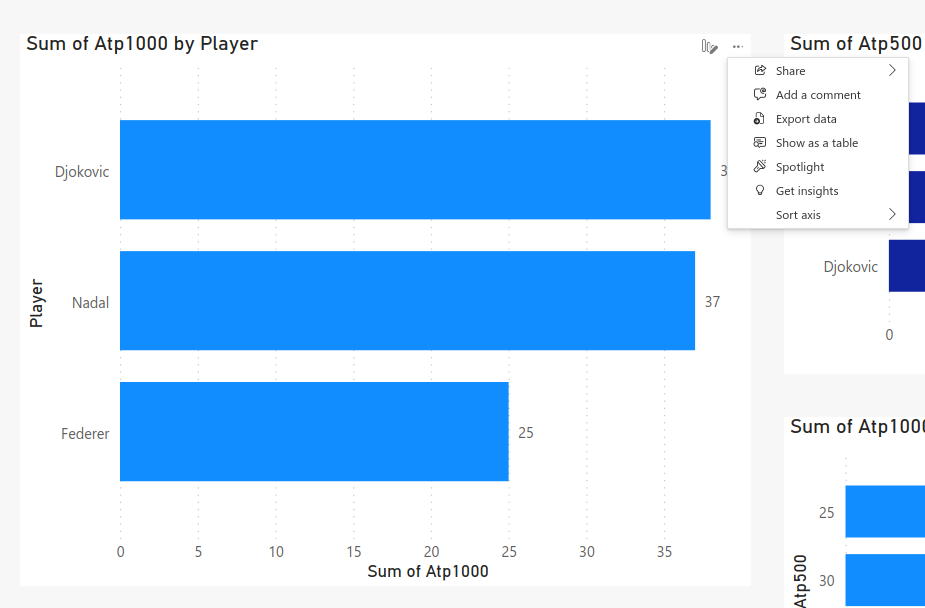
\includegraphics[width=\linewidth, height=7cm]{fig/eport.png}
    \caption{An example of the options bar for a visualization.}
    \label{fig:eport}
\end{figure}

\subsection*{What counts as different?}

If all rows are identical then the data are considered \emph{the same}. Additionally, being the same is invariant to permutations of columns and/or rows. However, the number of rows (columns) must match or the data are considered \emph{different}.
\par
Once the data are matched by reordering the rows and/or columns, every difference counts as being different and should be reported, regardless of the language, currency, metric, etc. In addition, if the values at both tables are numerical, their difference in value should be reported.

\section*{Software and algorithms}
We developed our solution in \textit{Python} and it is composed of two main parts\: data extraction and data comparison. \textbf{Data extraction} inputs two \textit{Power BI} reports uploaded to the \textit{Azure server}, along with the required credentials, and outputs a list of tables representing the data used for the visualizations. \textbf{Data comparison} compares the data and generates a report in \textit{Excel}. The software has a command line interface with the following arguments: \textbf{username} -- the username of the user's account on \textit{Azure server}, \textbf{password} -- the user's password, \textbf{gropuid1} -- the \textit{id} of the workspace where the first report is uploaded, \textit{reportid1} -- the \textit{id} of the first report, \textbf{gropuid2} -- the \textit{id} of the workspace where the second report is uploaded, \textit{reportid2} -- the \textit{id} of the second report, \textbf{data-folder} -- the path to the folder where the data will be stored. 


\subsection*{Data extraction}

For the first part, we tried several approaches to extract the data. One of them was by using the \textit{Power BI API} which was developed by \textit{Microsoft} for interacting with the server where the \textit{Power BI} reports are stored. Unfortunately, the API's functionalities are not sufficient, since it does not provide information about each visualization separately, but only with the dataset used for the whole report. The data for each visualization is calculated from that dataset, but the API does not provide the calculation formula. Another approach would be by extracting directly from the \textit{Power BI} file (PBIX). But, this approach is more complicated since Power BI queries the data every time it starts, so the data are stored in memory and removed when we close the report, which would also require manual interaction.
To extract the data we implemented a crawler using \textit{Selenium}, where we detect the position of each visualization at each page of the report and click on the \textit{More options} button in order to finally export the needed data for comparison. In addition, since the button is not always at the upper right corner, we also have the functionality of the crawler to try to find the button at the bottom right corner, if the button is not found at these two positions, it is considered that this is not a visualization that is created from data and thus not our objective for comparison.
\par
The main problem with this part of the software was how to automatically locate each visualization of the report. In order to solve the aforementioned challenge we developed an \hyperlink{algo1}{algorithm} that is using image processing methods on a screenshot of the \textit{Power BI} report.
\par

An important assumption is that the background of each visualization will always be white, and the background of the \textit{Power BI} report will always be of some colour that has high brightness. The main reason that we opted for this approach is the fact that most useful reports give more importance to the charts, pies, plots, and tables and they are usually with darker colours and in contrast to the background of the visualization, and often the colour considered to be as a background is white. Regarding the background of the report, usually, people who work with data analyses do not give too much importance to the background color and they usually left to the default light gray colour, since using much darker colours would give unnecessary high contrast.


\subsection*{Data comparison}
Once the data are downloaded, we must check if a reordering exists so that the data match. We developed the following \hyperlink{algo2}{algorithm}. With the described greedy approach, we sorted the instances based on how similar they are with respect to how many values are matched, and the result is the best possible matching between the tables without knowing their key values. After the rearrangement of the data instances, we simply compare each instance of the data between each visual where we defined several possible outcomes that we interpret as differences. 
\begin{itemize}
    \item Only one value is a string.
     \item Both values are strings, but they are different.
     \item One of the values is undefined. 
     \item Different values and/or currency.
\end{itemize}

Everything else is considered to as an identical value. Another aspect here is the definition of a currency, here we defined the value to be a currency where the currency sign is either immediately before the numerical value or to be concatenated after the numerical number with one space (' '), everything else is interpreted as a string value or a mistake in the defining the value with currency.
\begin{algorithm}

\caption{\hypertarget{algo1}{Localization of the visualizations.}}
\begin{enumerate}
\item Get a screenshot of the report using the \textit{Selenium} library.
\item Convert the image to a grayscale image.
\item Change each pixel that has a value lower than \\ 240 to value 255 (white colour).
\item Change the rest values that are not 255 to black.\\ At this point we have an image \\of only black and white pixels.
\item Find the contours in the image by using \\an algorithm proposed by Suzuki S. \cite{SUZUKI198532} \\which was implemented at the \textit{OpenCV} \cite{opencv_library} library.
\item By using the Douglas–Peucker algorithm that will connect the segments if they formed a line, \\we extract all possible rectangles from the image.
\item All rectangles that are close to the edges \\of the image are removed, along with rectangles \\that are too small.
    \item  Finally, we return for each rectangle its \\ (x, y) position along with its width and height.
\end{enumerate}

\end{algorithm}
\begin{algorithm}
\caption{\hypertarget{algo2}{Rearrangement of the data instances}}
\begin{enumerate}
    \item Initialize two new tables.
    \item Rearrange the columns in both tables in such \\way that, first are the columns that are mutual \\and then the rest.
    \item Find the pair of instances (one from the first and another from the second table), that have the most values matched between them.
    \item Add both instances to the new tables.
    \item Repeat the process from 2 to 4 until \\one of the tables is empty.
    \item  Move the left data instances to the bottom of the corresponding new table.
\end{enumerate}

\end{algorithm}

\subsection*{Results output}
 The result that we focused on was an \textit{Excel} report Fig. \ref{fig:report2} that will have the same number of pages as the \textit{Power BI} report with an additional page which will represent the \textit{Overview} Fig. \ref{fig:overall} comparison between each pair of visualizations from the reports. In addition, it is implemented a link to the comparison in the report for each pair of visualizations, which links to the page with the detailed comparison. Then, on each page for every pair of visualizations, the data used for creation is presented, along with the corresponding number of rows and columns and their differences. In addition, the cells showing the differences are coloured red (different) or green (the same). The code and instructions on how to use it can be found here: \url{https://github.com/theteleton/project}.

\begin{figure}
    \centering
    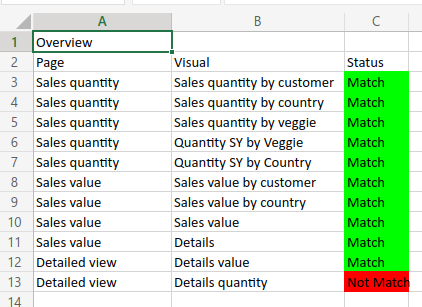
\includegraphics[width=\linewidth, height=6.5cm]{fig/overview.png}
    \caption{The \textit{Overview} part of the comparison report.}
    \label{fig:overall}
\end{figure}
%------------------------------------------------

%------------------------------------------------
\begin{figure*}
      \centering
    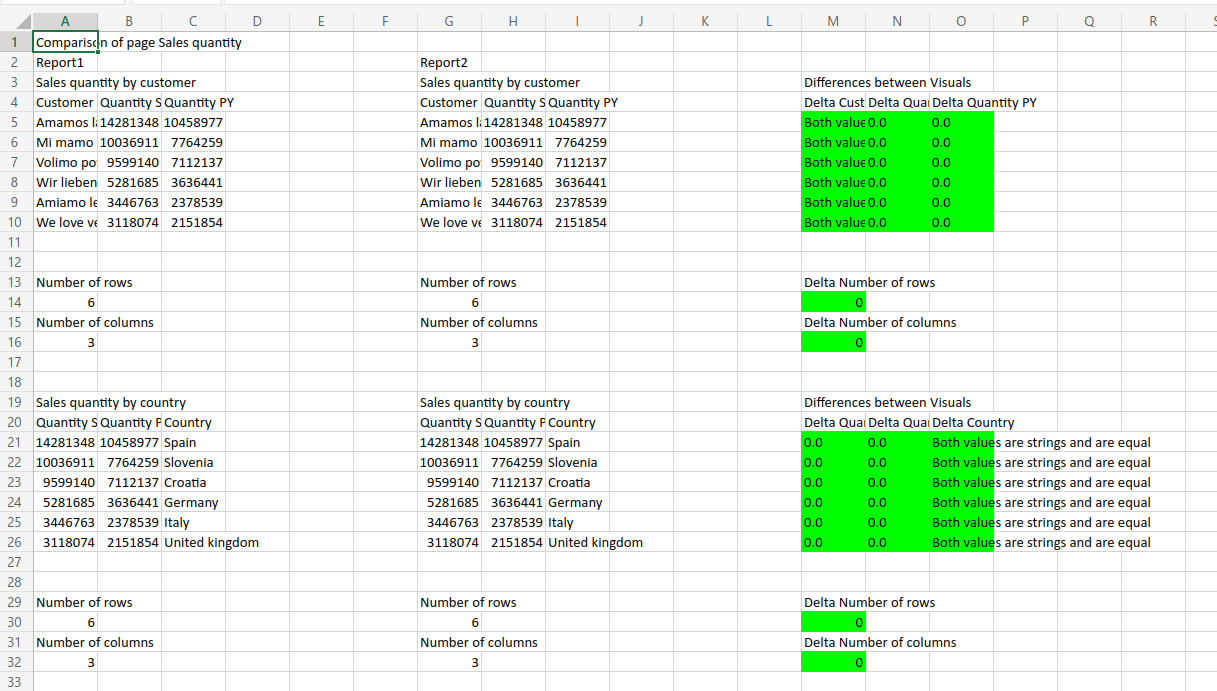
\includegraphics[width=\linewidth, height=10cm]{fig/best_report.png}
    \caption{An example of a page from a comparison of several equal visualizations.}
    \label{fig:report2}  
\end{figure*}

\section*{Discussion}
We achieved the main objective of our work. We implemented software that \textbf{automatically} locates each visualization on every page from the report and is generating a comparison report showing the differences between each pair of visualizations. As far as we are aware, this is the first software that does this. Since it is fully automated the software without any human assistance can process as much pair of reports as possible in a respected time span and generate for each pair an comparison report. This functionality is also parallelizable, which can be further useful it can process pairs much faster than a human expert could. Processing a pair is also trivially parallelizable.
\par

Our solution has limitations. \textbf{That it increases linearly with number of visualizations is not a limitation, it has to increase at least linearly, because at a minumum, we have to go through each visualization at least once.} The assumptions about the visualization and background colours could be lifted by developing a more robust segmentation algorithm, most likely based on deep neural networks. Rearrangement of the data has time complexity of $O(n^3)$, where $n$ is the number of instances, which would be a problem for large $n$. If we calculate beforehand, the maximum number of matching between the instances, we can stop the search when we find the best match. Assuming that most  instances will be matched as best as possible most of the time,  we can improve the complexity to quadratic.

\In addition, there might be also a way to bypass the need to click on each \textit{Export data} button to get the data by getting the data at the moment when they are loaded at memory (when using the Power BI desktop software). But this method would require more research and knowledge of the architecture of the \textit{Power BI} software.



\section*{Acknowledgments}

I would like to thank the \textbf{DataScience@UL-FRI} initiative for providing the Project course as part of the Data Science Master's program. I would also like to thank  \textbf{In516ht} and especially Vid Smrke for taking part in the \textit{Project Competition} and providing data and advice.  And finally, I want to thank prof. dr. Erik \v{S}trumbelj for the guidance and responsiveness during the competition.



%----------------------------------------------------------------------------------------
%	REFERENCE LIST
%----------------------------------------------------------------------------------------
\bibliographystyle{unsrt}
\bibliography{report}

\end{document}